\section{Experiments \& Results}
\label{sec:experiments}

\subsection{Training Setup}
Our training process involves first training the feature prediction network
on its own, followed by training a modified WaveNet independently on the outputs
generated by the first network.

To train the feature prediction network, we apply the standard
maximum-likelihood training procedure (feeding in the
correct output instead of the predicted output on the decoder side, also
referred to as {\em teacher-forcing})
with a batch size of 64 on a single GPU. We use the Adam optimizer
\cite{DBLP:journals/corr/KingmaB14} with
$\beta_1=0.9, \beta_2=0.999, \epsilon=10^{-6}$ and a learning rate of
$10^{-3}$ exponentially decaying to $10^{-5}$ starting after 50,000 iterations.
We also apply $L_2$ regularization with weight $10^{-6}$.

We then train our modified WaveNet on the \emph{ground truth-aligned}
predictions of the feature prediction network.
That is, the prediction network is run in teacher-forcing mode,
where each predicted frame is conditioned on the encoded input sequence and the
corresponding previous frame in the ground truth spectrogram. This ensures that
each predicted frame exactly aligns with the target waveform samples.

We train with a batch size of 128 distributed across 32 GPUs
with synchronous updates, using the Adam optimizer with
$\beta_1=0.9, \beta_2=0.999, \epsilon=10^{-8}$ and a fixed learning rate of
$10^{-4}$. It helps quality to average model weights over recent updates.  Therefore
we maintain an exponentially-weighted moving average of the network parameters
over update steps with a decay of 0.9999 -- this version is used for inference
(see also \cite{DBLP:journals/corr/KingmaB14}).
%
To speed up convergence, we scale the waveform targets by a factor of $127.5$
which brings the initial outputs of the mixture of logistics layer closer to
the eventual distributions.

We train all models on an internal US English dataset\cite{46150}, which
contains 24.6 hours of speech from a single professional female speaker.
%
All text in our datasets is spelled out. \eg ``16'' is written as ``sixteen'',
\ie our models are all trained on normalized text.

\subsection{Evaluation}

When generating speech in inference mode, the ground truth targets are
not known.  Therefore, the predicted outputs from the previous step
are fed in during decoding, in contrast to the teacher-forcing
configuration used for training.

We randomly selected 100 fixed examples from the test set of our internal
dataset as the evaluation set.
Audio generated on this set are sent to a human rating service similar to
Amazon's Mechanical Turk where each sample is rated by at least 8 raters on a
scale from 1 to 5 with 0.5 point increments, from which a subjective mean opinion score
(MOS) is calculated. Each evaluation is conducted independently from each other,
so the outputs of two different models are not directly compared when
raters assign a score to them.

Note that while instances in the evaluation set never appear in the training
set, there are some recurring patterns and common words between the two sets.
While this could potentially result in an inflated MOS compared to
an evaluation set consisting of sentences generated from random words, using
this set allows us to compare to the ground truth.  Since all the systems
we compare are trained on the same data, relative comparisons are still
meaningful.

Table \ref{tbl:mos_various_systems} shows
a comparison of our method against various prior systems.
In order to better isolate the effect of using mel spectrograms as features,
we compare to a WaveNet conditioned on linguistic features\cite{45774} with similar
modifications to the WaveNet architecture as introduced above. We also compare
to the original
Tacotron that predicts linear spectrograms and uses Griffin-Lim to synthesize
audio, as well as concatenative \cite{gonzalvo2016recent} and parametric
\cite{zen2016fast} baseline systems, both of which have been used in production at Google.
%
% It's important to highlight the main result of the paper!
We find that the proposed system significantly outpeforms all other TTS systems,
and results in an MOS comparable to that of the ground truth audio.
\footnote[2]{Samples available at https://google.github.io/tacotron/publications/tacotron2.}

\begin{table}[H]
  \centering
  \begin{tabular}{lc}
  \toprule
  System                & MOS \\
  \midrule
  Parametric            & $3.492 \pm 0.096$   \\
  Tacotron (Griffin-Lim)& $4.001 \pm 0.087$   \\
  Concatenative         & $4.166 \pm 0.091$   \\
  WaveNet (Linguistic)  & $4.341 \pm 0.051$   \\
  Ground truth          & $4.582 \pm 0.053$   \\
  \midrule
  Tacotron~2 (this paper)& \bm{$4.526 \pm 0.066$}   \\
  \bottomrule
  \end{tabular}
\caption{Mean Opinion Score (MOS) evaluations with 95\% confidence intervals
computed from the t-distribution for various systems.}
\label{tbl:mos_various_systems}
\end{table}

We also conduct a side-by-side evaluation between audio synthesized by
our system and the ground truth.
%
For each pair of utterances, raters are asked to give a score ranging from -3
(synthesized much worse than ground truth) to 3 (synthesized much better than
ground truth).
%
The overall mean score of $-0.270 \pm 0.155$ shows that raters have a small but
statistically significant preference towards ground truth over our results.
%
See Figure~\ref{fig:sxs_breakdown} for a detailed breakdown.
%
The comments from raters indicate that occasional mispronunciation by our
system is the primary reason for this preference.

\begin{figure}[H]
\centering
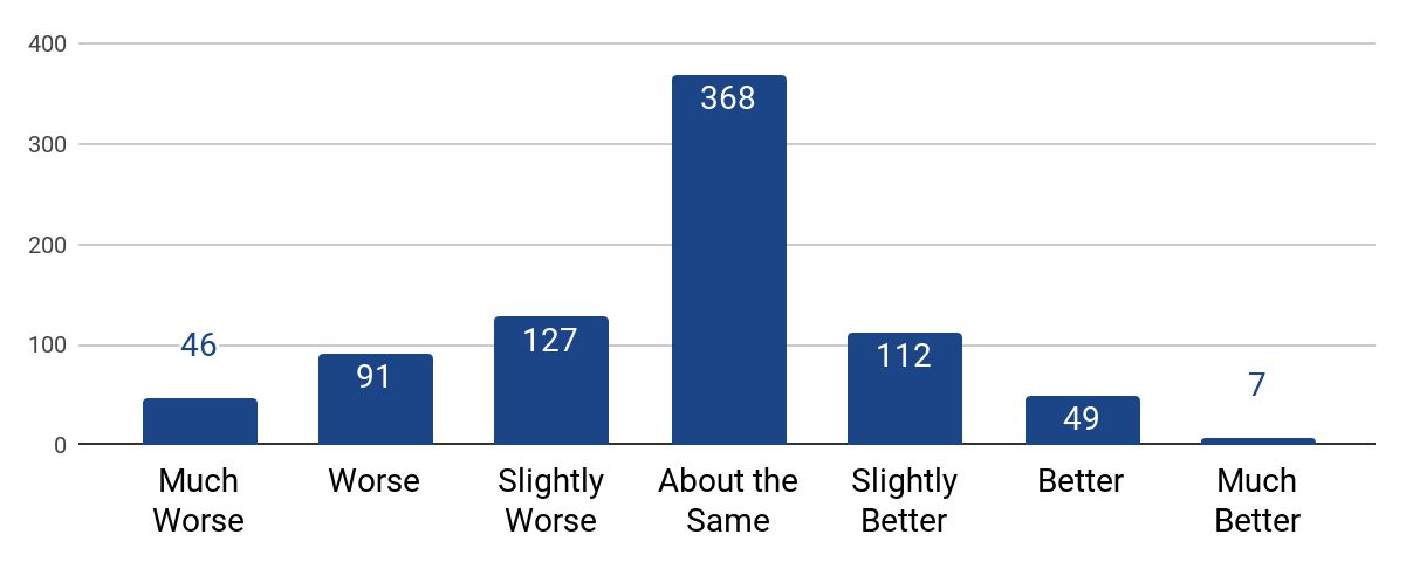
\includegraphics[scale=0.35]{sxs-breakdown.pdf}
\caption{Synthesized vs. ground truth: 800 ratings on 100 items.}
\label{fig:sxs_breakdown}
\end{figure}

We ran a separate rating experiment on the custom 100-sentence test set from
Appendix E of \cite{2017arXiv171007654P}, obtaining a MOS of 4.354.
In a manual analysis of the error modes of our system, counting errors in
each category independently, 0 sentences contained repeated words,
6 contained mispronunciations, 1 contained skipped words, and 23 were
subjectively decided to contain unnatural prosody, such as emphasis on the
wrong syllables or words, or unnatural pitch. End-point prediction failed in a
single case, on the input sentence containing the most characters.
These results show that while our system is able to reliably attend to the
entire input, there is still room for improvement in prosody modeling.

Finally, we evaluate samples generated from 37 news headlines to test the
generalization ability of our system to out-of-domain text. On this task, our
model receives a MOS of $4.148 \pm 0.124$ while WaveNet conditioned on
linguistic features receives a MOS of $4.137 \pm 0.128$.
A side-by-side evaluation comparing the output of these systems also
shows a virtual tie -- a statistically insignificant preference towards our
results by $0.142 \pm 0.338$. Examination of rater comments shows that our
neural system tends to generate speech that feels more natural and human-like,
but it sometimes runs into pronunciation difficulties, \eg when
handling names. This result points to a challenge for end-to-end
approaches -- they require training on data that cover intended usage.

\subsection{Ablation Studies}
\label{sec:ablation}

\subsubsection{Predicted Features versus Ground Truth}
\label{ssec:gtfeats}

While the two components of our model were trained separately, the WaveNet component
depends on the predicted features for training. An alternative
is to train WaveNet independently on mel spectrograms extracted from ground
truth audio. We explore this in Table~\ref{tbl:pred_gt}.

\begin{table}[H]
  \centering
  \begin{tabular}{lcc}
    \toprule
                 & \multicolumn{2}{c}{Synthesis}\\
    Training     & Predicted         & Ground truth \\
    \midrule
    Predicted    & $4.526 \pm 0.066$ & $4.449 \pm 0.060$ \\
    Ground truth & $4.362 \pm 0.066$ & $4.522 \pm 0.055$ \\
    \bottomrule
  \end{tabular}
\caption{Comparison of evaluated MOS for our system when WaveNet trained on
predicted/ground truth mel spectrograms are made to synthesize from
predicted/ground truth mel spectrograms.}
\label{tbl:pred_gt}
\end{table}

As expected, the best performance is obtained when the features used for
training match those used for inference. However, when trained on
ground truth features and made to synthesize from
predicted features, the result is worse than the opposite.
This is due to the tendency of the predicted spectrograms to be oversmoothed and less
detailed than the ground truth -- a consequence of the squared error loss
optimized by the feature prediction network. When trained on ground truth
spectrograms, the network does not learn to generate high quality speech
waveforms from oversmoothed features.


\subsubsection{Linear Spectrograms}
\label{ssec:linear}

Instead of predicting mel spectrograms, we experiment with training
to predict linear-frequency spectrograms instead, making it
possible to invert the spectrogram using Griffin-Lim.

\begin{table}[H]
  \centering
  \begin{tabular}{lc}
  \toprule
  System                        & MOS \\
  \midrule
  Tacotron~2 (Linear + G-L)     & $3.944 \pm 0.091$   \\
  Tacotron~2 (Linear + WaveNet) & $4.510 \pm 0.054$   \\
  Tacotron~2 (Mel + WaveNet)    & $\bm{4.526 \pm 0.066}$ \\
  \bottomrule
  \end{tabular}
\caption{Comparison of evaluated MOS for Griffin-Lim vs. WaveNet as a vocoder,
and using 1,025-dimensional linear spectrograms vs. 80-dimensional
mel spectrograms as conditioning inputs to WaveNet.}
\end{table}

As noted in \cite{DBLP:journals/corr/ArikDGMPPRZ17}, WaveNet produces much
higher quality audio compared to Griffin-Lim. However, there is not much
difference between the use of linear-scale or mel-scale spectrograms. As such,
the use of mel spectrograms seems to be a strictly better choice since it is a
more compact representation. It would be interesting to explore the
trade-off between the number of mel frequency bins versus audio quality
in future work.


\subsubsection{Post-Processing Network}
\label{ssec:postedit}

%In Tacotron, the post-processing network was used to convert the prediction
%targets to linear spectrograms so that they could be inverted using Griffin-Lim.
Since it is not possible to use the information of predicted future frames
before they have been decoded, we use a convolutional post-processing network
to incorporate past and future frames after decoding to improve the feature
predictions. However, because WaveNet already contains convolutional layers,
one may wonder if the post-net is still necessary when WaveNet is used as the
vocoder. To answer this
question, we compared our model with and without the post-net, and found that
without it, our model only obtains a MOS score of $4.429 \pm 0.071$, compared to
$4.526 \pm 0.066$ with it, meaning that empirically the post-net is still an
important part of the network design.


\subsubsection{Simplifying WaveNet}
\label{ssec:simplifywavenet}

A defining feature of WaveNet is its use of dilated convolution to increase
the receptive field exponentially with the number of layers.
%
We evaluate models with varying receptive field sizes and number of
layers to test our hypothesis that a shallow network with a small receptive
field may solve the problem satisfactorily since mel spectrograms are a much
closer representation of the waveform than linguistic features and already
capture long-term dependencies across frames.

As shown in Table \ref{tbl:wavenets}, we find that our model can generate
high-quality audio using as few as 12 layers with a receptive field of
10.5~ms, compared to 30 layers and 256~ms in the baseline model. These
results confirm the observations in \cite{DBLP:journals/corr/ArikCCDGKLMRSS17}
that a large receptive field size is not an essential factor for audio
quality. However, we hypothesize that it is the choice to condition on mel
spectrograms that allows this reduction in complexity.

On the other hand, if we eliminate dilated convolutions altogether, the
receptive field becomes two orders of magnitude smaller than the baseline and
the quality degrades significantly even though the stack is as deep as the
baseline model.
%
This indicates that the model requires sufficient context at the time scale of
waveform samples in order to generate high quality sound.

\begin{table}[H]
  \centering
  \begin{tabular}{ccccc}
  \toprule
  \makecell{Total\\layers} & \makecell{Num\\cycles} &
  \makecell{Dilation\\cycle size} & \makecell{Receptive field\\(samples / ms)} &
  MOS \\
  \midrule
  30 & 3  & 10 & 6,139 / 255.8 & $4.526 \pm 0.066$   \\
% 30 & 5  &  6 & 631 / 26.3 & $4.518 \pm 0.057$  \\
  24 & 4 &  6 & 505 / 21.0 & $4.547 \pm 0.056$   \\
% 18 & 3 &  6 & 379 / 15.8 & $4.515 \pm 0.058$   \\
  12 & 2 &  6 & 253 / 10.5 & $4.481 \pm 0.059$   \\
  30 & 30 &  1 & 61 / 2.5 & $3.930 \pm 0.076$ \\
  \bottomrule
  \end{tabular}
\caption{WaveNet with various layer and receptive field sizes.}
\label{tbl:wavenets}
\end{table}
